\documentclass{beamer}
\usetheme{metropolis}           % Use metropolis theme
\usepackage[spanish]{babel}
\usepackage{amsmath,mathtools,array}
\usepackage{amssymb} 
\usepackage{amsthm} 
\usepackage{tikz}
\usepackage{microtype}
% \usepackage{../paper/paper}

\title{First steps towards a formalization of Forcing}
\author{Emmanuel Gunther\and \emph{Miguel Pagano}\and Pedro Sánchez Terraf}
\date{LSFA - Fortaleza, 26 September 2018}
\usepackage{amsmath}
%\usepackage{amsthm}
\usepackage{amsfonts}
\usepackage{amssymb}
%\usepackage{bbm}  % Para el \bb{1}
%\usepackage[numbers]{natbib}
\usepackage{enumitem}
\usepackage{babel}
%\usepackage{babelbib}
\usepackage{multidef}
\usepackage{verbatim}
\usepackage{stmaryrd} %% para \llbracket
%%
%% \usepackage[bottom=2cm, top=2cm, left=2cm, right=2cm]{geometry}
%% \usepackage{titling}
%% \setlength{\droptitle}{-10ex} 
%%
\renewcommand{\o}{\vee}
\renewcommand{\O}{\bigvee}
\newcommand{\y}{\wedge}
\newcommand{\Y}{\bigwedge}
\newcommand{\limp}{\rightarrow}
\newcommand{\lsii}{\leftrightarrow}
%%

\DeclareMathOperator{\cf}{cf}
\DeclareMathOperator{\dom}{dom}
\DeclareMathOperator{\im}{img}
\DeclareMathOperator{\Fn}{Fn}
\DeclareMathOperator{\rk}{rk}
\DeclareMathOperator{\mos}{mos}
\DeclareMathOperator{\trcl}{trcl}
\DeclareMathOperator*{\diag}{\bigtriangleup}
\DeclareMathOperator{\Con}{Con}
\DeclareMathOperator{\Club}{Club}


\newcommand{\modelo}[1]{\mathbf{#1}}
\newcommand{\axiomas}[1]{\mathit{#1}}
\newcommand{\clase}[1]{\mathsf{#1}}
\newcommand{\poset}[1]{\mathbb{#1}}
\newcommand{\operador}[1]{\mathbf{#1}}

%% \newcommand{\Lim}{\clase{Lim}}
%% \newcommand{\Reg}{\clase{Reg}}
%% \newcommand{\Card}{\clase{Card}}
%% \newcommand{\On}{\clase{On}}
%% \newcommand{\WF}{\clase{WF}}
%% \newcommand{\HF}{\clase{HF}}
%% \newcommand{\HC}{\clase{HC}}
%%
%% El siguiente comando reemplaza todos los anteriores:
%%
\multidef{\clase{#1}}{Card,HC,HF,Lim,On->Ord,Reg,WF,Ord}
\newcommand{\ON}{\On}

%% En lugar de usar todo el paquete bbm:
\DeclareMathAlphabet{\mathbbm}{U}{bbm}{m}{n} 
\newcommand{\1}{\mathbbm{1}}

%%
%% \newcommand{\calD}{\mathcal{D}}
%% \newcommand{\calS}{\mathcal{S}}
%% \newcommand{\calU}{\mathcal{U}}
%% \newcommand{\calB}{\mathcal{B}}
%% \newcommand{\calL}{\mathcal{L}}
%% \newcommand{\calF}{\mathcal{F}}
%% \newcommand{\calT}{\mathcal{T}}
%% \newcommand{\calW}{\mathcal{W}}
%% \newcommand{\calA}{\mathcal{A}}
%%
%% El siguiente comando reemplaza todos los anteriores:
%%
\multidef[prefix=cal]{\mathcal{#1}}{A-Z}
%%
%% \newcommand{\A}{\modelo{A}}
%% \newcommand{\BB}{\modelo{B}}
%% \newcommand{\ZZ}{\modelo{Z}}
%% \newcommand{\PP}{\modelo{P}}
%% \newcommand{\QQ}{\modelo{Q}}
%% \newcommand{\RR}{\modelo{R}}
%%
%% El siguiente comando reemplaza todos los anteriores:
%%
\multidef{\modelo{#1}}{A,BB->B,CC->C,NN->N,PP->P,QQ->Q,RR->R,ZZ->Z}

\multidef[prefix=p]{\mathbb{#1}}{A-Z}
%% \newcommand{\B}{\modelo{B}}
%% \newcommand{\C}{\modelo{C}}
%% \newcommand{\F}{\modelo{F}}
%% \newcommand{\D}{\modelo{D}}

\newcommand{\Th}{\mb{Th}}
\newcommand{\Mod}{\mb{Mod}}

\newcommand{\Se}{\operador{S^\prec}}
\newcommand{\Pu}{\operador{P_u}}
\renewcommand{\Pr}{\operador{P_R}}
\renewcommand{\H}{\operador{H}}
\renewcommand{\S}{\operador{S}}
\newcommand{\I}{\operador{I}}
\newcommand{\E}{\operador{E}}

\newcommand{\se}{\preccurlyeq}
\newcommand{\ee}{\succ}
\newcommand{\id}{\approx}
\newcommand{\subm}{\subseteq}
\newcommand{\ext}{\supseteq}
\newcommand{\iso}{\cong}
%%
\renewcommand{\emptyset}{\varnothing}
\newcommand{\rel}{\mathcal{R}}
\newcommand{\Pow}{\mathop{\mathcal{P}}}
\renewcommand{\P}{\Pow}
\newcommand{\BP}{\mathrm{BP}}
\newcommand{\func}{\rightarrow}
\newcommand{\ord}{\mathrm{Ord}}
\newcommand{\R}{\mathbb{R}}
\newcommand{\N}{\mathbb{N}}
\newcommand{\Z}{\mathbb{Z}}
\renewcommand{\I}{\mathbb{I}}
\newcommand{\Q}{\mathbb{Q}}
\newcommand{\B}{\mathbf{B}}
\newcommand{\<}{\langle}
\renewcommand{\>}{\rangle}
\newcommand{\lb}{\langle}
\newcommand{\rb}{\rangle}
\newcommand{\impl}{\rightarrow}
\newcommand{\ent}{\Rightarrow}
\newcommand{\tne}{\Leftarrow}
\newcommand{\sii}{\Leftrightarrow}
\renewcommand{\phi}{\varphi}
\newcommand{\phis}{{\varphi^*}}
\renewcommand{\th}{\theta}
\newcommand{\Lda}{\Lambda}
\newcommand{\La}{\Lambda}
\newcommand{\lda}{\lambda}
\newcommand{\ka}{\kappa}
\newcommand{\del}{\delta}
\newcommand{\de}{\delta}
\newcommand{\ze}{\zeta}
%\newcommand{\ }{\ }
\newcommand{\la}{\lambda}
\newcommand{\al}{\alpha}
\newcommand{\be}{\beta}
\newcommand{\ga}{\gamma}
\newcommand{\Ga}{\Gamma}
\newcommand{\ep}{\varepsilon}
\newcommand{\De}{\Delta}
\newcommand{\defi}{\mathrel{\mathop:}=}
\newcommand{\forces}{\Vdash}
%\newcommand{\ap}{\mathbin{\wideparen{\ }}}
\newcommand{\Tree}{{\mathrm{Tr}_\N}}
\newcommand{\PTree}{{\mathrm{PTr}_\N}}
\newcommand{\NWO}{\mathit{NWO}}
\newcommand{\Suc}{{\N^{<\N}}}%
\newcommand{\init}{\mathsf{i}}
\newcommand{\ap}{\mathord{^\smallfrown}}
\newcommand{\Cantor}{\mathcal{C}}
%\newcommand{\C}{\Cantor}
\newcommand{\Baire}{\mathcal{N}}
\newcommand{\sig}{\ensuremath{\sigma}}
\newcommand{\fsig}{\ensuremath{F_\sigma}}
\newcommand{\gdel}{\ensuremath{G_\delta}}
\newcommand{\Sig}{\ensuremath{\boldsymbol{\Sigma}}}
\newcommand{\bPi}{\ensuremath{\boldsymbol{\Pi}}}
\newcommand{\Del}{\ensuremath{\boldsymbol\Delta}}
%\renewcommand{\F}{\operador{F}}
\newcommand{\ths}{{\theta^*}}
\newcommand{\om}{\ensuremath{\omega}}
%\renewcommand{\c}{\complement}
\newcommand{\comp}{\mathsf{c}}
\newcommand{\co}[1]{\left(#1\right)^\comp}
\newcommand{\len}[1]{\left|#1\right|}
\DeclareMathOperator{\tlim}{\overline{\mathrm{TLim}}}
\newcommand{\card}[1]{{\left|#1\right|}}
\newcommand{\bigcard}[1]{{\bigl|#1\bigr|}}
%
% Cardinality
%
\newcommand{\lec}{\leqslant_c}
\newcommand{\gec}{\geqslant_c}
\newcommand{\lc}{<_c}
\newcommand{\gc}{>_c}
\newcommand{\eqc}{=_c}
\newcommand{\biy}{\approx}
\newcommand*{\ale}[1]{\aleph_{#1}}
%
\newcommand{\Zerm}{\axiomas{Z}}
\newcommand{\ZC}{\axiomas{ZC}}
\newcommand{\AC}{\axiomas{AC}}
\newcommand{\DC}{\axiomas{DC}}
\newcommand{\MA}{\axiomas{MA}}
\newcommand{\CH}{\axiomas{CH}}
\newcommand{\ZFC}{\axiomas{ZFC}}
\newcommand{\ZF}{\axiomas{ZF}}
\newcommand{\Inf}{\axiomas{Inf}}
%
% Cardinal characteristics
%
\newcommand{\cont}{\mathfrak{c}}
\newcommand{\spl}{\mathfrak{s}}
\newcommand{\bound}{\mathfrak{b}}
\newcommand{\mad}{\mathfrak{a}}
\newcommand{\tower}{\mathfrak{t}}
%
\renewcommand{\hom}[2]{{}^{#1}\hskip-0.116ex{#2}}
\newcommand{\pred}[1][{}]{\mathop{\mathrm{pred}_{#1}}}
%% Postfix operator with supressable space:
%% \newcommand*{\iseg}{\relax\ifnum\lastnodetype>0 \mskip\medmuskip\fi{\downarrow}} %
\newcommand*{\iseg}{{\downarrow}}
\newcommand{\rr}{\mathrel{R}}
\newcommand{\restr}{\upharpoonright}
%\newcommand{\type}{\mathtt{}}
\newcommand{\app}{\mathop{\mathrm{Aprox}}}
\newcommand{\hess}{\triangleleft}
\newcommand{\bx}{\bar{x}}
\newcommand{\by}{\bar{y}}
\newcommand{\bz}{\bar{z}}
\newcommand{\union}{\mathop{\textstyle\bigcup}}
\newcommand{\sm}{\setminus}
\newcommand{\sbq}{\subseteq}
\newcommand{\nsbq}{\subseteq}
\newcommand{\mty}{\emptyset}
\newcommand{\dimg}{\text{\textup{``}}} % direct image
\newcommand{\quine}[1]{\ulcorner{\!#1\!}\urcorner}
%\newcommand{\ntrm}[1]{\textsl{\textbf{#1}}}
\newcommand{\Null}{\calN\!\mathit{ull}}
\DeclareMathOperator{\club}{Club}
\DeclareMathOperator{\otp}{otp}

%%%%%%%%%%%%%%%%%%%%%%%%%
% Variant aleph, beth, etc
% From http://tex.stackexchange.com/q/170476/69595
\makeatletter
\@ifpackageloaded{txfonts}\@tempswafalse\@tempswatrue
\if@tempswa
  \DeclareFontFamily{U}{txsymbols}{}
  \DeclareFontFamily{U}{txAMSb}{}
  \DeclareSymbolFont{txsymbols}{OMS}{txsy}{m}{n}
  \SetSymbolFont{txsymbols}{bold}{OMS}{txsy}{bx}{n}
  \DeclareFontSubstitution{OMS}{txsy}{m}{n}
  \DeclareSymbolFont{txAMSb}{U}{txsyb}{m}{n}
  \SetSymbolFont{txAMSb}{bold}{U}{txsyb}{bx}{n}
  \DeclareFontSubstitution{U}{txsyb}{m}{n}
  \DeclareMathSymbol{\aleph}{\mathord}{txsymbols}{64}
  \DeclareMathSymbol{\beth}{\mathord}{txAMSb}{105}
  \DeclareMathSymbol{\gimel}{\mathord}{txAMSb}{106}
  \DeclareMathSymbol{\daleth}{\mathord}{txAMSb}{107}
\fi
\makeatother

%%%%%%%%%%%%%%%%%%%%%%%%%%%%%%%%%%%%%%%%%%%%%%%%%%%%%%%%%%%%
%%
%% Theorem Environments
%%
%% \newtheorem{theorem}{Theorem}
%% \newtheorem{lemma}[theorem]{Lemma}
%% \newtheorem{prop}[theorem]{Proposition}
%% \newtheorem{corollary}[theorem]{Corollary}
%% \newtheorem{claim}{Claim}
%% \newtheorem*{claim*}{Claim}
%% \theoremstyle{definition}
%% \newtheorem{definition}[theorem]{Definition}
%% \newtheorem{remark}[theorem]{Remark}
%% \newtheorem{example}[theorem]{Example}
%% \theoremstyle{remark}
%% \newtheorem*{remark*}{Remark}
%%
%%%%%%%%%%%%%%%%%%%%%%%%%%%%%%%%%%%%%%%%%%%%%%%%%%%%%%%%%%%%%%%%%%%%%%

%% \newenvironment{inducc}{\begin{list}{}{\itemindent=2.5em \labelwidth=4em}}{\end{list}}
%% \newcommand{\caso}[1]{\item[\fbox{#1}]}
\newenvironment{proofofclaim}{\begin{proof}[Proof of Claim]}{\end{proof}}


%%% Local Variables: 
%%% mode: latex
%%% TeX-master: "first_steps_into_forcing"
%%% End: 

\usepackage{../isabelle}
\usepackage{../isabellesym}
\begin{document}

\maketitle
%% Outline
% 

\begin{frame}{Zermelo-Fraenkel Set Theory}
  \begin{block}{}
    Set theory arose at the early twentieth century as one
    possible foundation for mathematics.
  \end{block}
  \begin{block}{}
    More formally, set theory is a first order theory ($ZFC$) with no
    constants and one relational symbol $\in$. % It has some axioms
    % (extensionality, pairing, foundation, union, powerset, infinity)
    % and two axiom schemes (separation and replacement). This theory
    % is known by $ZF$; while $ZFC$ is $ZF$ plus the axiom of Choice.
  \end{block}
  \begin{block}{}
    To say that $ZFC$ is a possible foundation for mathematics means
    that any mathematical theorem, say $T$, can be deduced from $ZFC$:
    \[ ZFC \vdash T \]
  \end{block}
\end{frame}
\begin{frame}{Cantor's Question and Gödel's and Cohen's answers}
  \begin{block}{}
    Cantor posed the \emph{Continuum Hypothesis} ($\CH$):
    \begin{quote}
      Every uncountable subset of $\R$ is equipotent with $\R$.
    \end{quote}
  \end{block}
  \begin{block}{}
    Gödel showed that $\CH$ is \emph{relatively consistent} with $ZFC$.
  \end{block}
  \begin{block}{}
    Later, Cohen showed that also the negation of $\CH$ is relatively
    consistent with $ZFC$. For this he invented the technique of
    \emph{forcing}.
  \end{block}
\end{frame}

\begin{frame}{Some preliminaries}
  \begin{block}{}
    To say that $T$ is \emph{relatively consistent} with $ZFC$ can be
    understood in two ways:
    \begin{enumerate}
    \item Construct a model $M'$ of $ZFC+T$ from a model $M$ for
      $ZFC$.
    \item Alternatively, deduce a contradiction in $ZFC$ from a
      contradiction in $ZFC+T$.% (Interestingly both proofs give
      % rise to algorithms for this)
    \end{enumerate}
  \end{block}

  \begin{block}{}
    Cohen's proofs construct a model $ZFC+\neg\CH$ assuming a
    countable and transitive model (ctm).
  \end{block}
  \begin{itemize}
  \item  $M$ is a \emph{transitive} model of $ZFC$ if $x \in M$ implies
    $x\subset M$.
  \item $M$ is \emph{countable} if it is equipotent with $\N$.
  \end{itemize}

  % \begin{block}{}
  %   Notice that it is fine to ask for a ctm because at the end we
  %   want to transforms contradictions 
  % \end{block}
\end{frame}

\begin{frame}{Forcing}
  \begin{block}{}
    \begin{itemize}
    \item Given a ctm $M$ and a \emph{generic} set $G$ \emph{for} $M$,
      one constructs a new ctm $M[G]$.
    \item One defines a poset $(P,\leq)$, where $P \in M$. The
      existence of a generic filter $G$ follows from Rasiowa-Sikorski.
    \item $M[G] = \{\val(G,x)\, |\, x \in M \}$ 
    \item Depending on the definition of $P$, $M[G]$ will satisfy
      $\CH$ or $\neg\CH$.
    \end{itemize}
  \end{block}
\end{frame}

\begin{frame}{Our goal: formalize forcing}
  \begin{block}{Questions?}
    \begin{itemize}
    \item Why forcing? Has not been formalized yet. % (Paulson formalized Gödel's result)
    \item Related work. Paulson formalized Gödel's proof. %is the largest development and
%      we can build on top of his work.
    \item Which proof assistant? Because of the previous answer:
      Isabelle/ZF.
    \end{itemize}
  \end{block}
\end{frame}

\begin{frame}{Isabelle/ZF}
  \begin{block}{Axiomatization of ZF in Isabelle/FOL}
    \begin{itemize}
    \item Sets are terms of type \isatt{i} and formulas have type
      \isatt{o}. % None of them are recursive data-types.
    \item Axioms of $ZFC$ are postulated as axioms of Isabelle:
      \isa{extension: A\ =\ B\ \isasymlongleftrightarrow\ A\ \isasymsubseteq\ B\ \isasymand\ B \isasymsubseteq\ A}
    \item A theorem of $ZFC$ is a \emph{lemma} of Isabelle/ZF:
           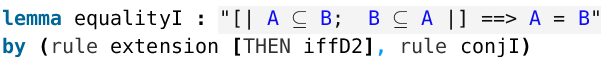
\includegraphics[scale=1.3]{eqI.png}
     \item In order to speak of formulas and satisfaction
           (models), Paulson coded formulas (and much more) as sets.
         \item He also defined relativized (to a class) versions of the axioms\\
\hspace{-0.5cm}   \isa{upair\_ax(M) == \isasymforall x[M]. \isasymforall  y[M].\isasymexists z[M]. upair(M,x,y,z)}
     \end{itemize}
\end{block}
\end{frame}

\begin{frame}{First steps towards Forcings}
  \begin{block}{Our strategy}
    \begin{enumerate}
    \item Be as modular as possible, using \emph{locales}.
    \item Define interfaces to deal with models of $ZFC$.
    \item Exploit the modularity of forcing to divide the work.
    \end{enumerate}
  \end{block}
\end{frame}

\begin{frame}{What have we done?}
  \begin{block}{Existence of a generic filter}
  \begin{itemize}
  \item Proved a principle of dependent choice.
  \item Using that principle, proved Rasiowa-Sikorski.
  \item If $M$ is a ctm and $P\in M$ is a poset, then
    there exists a generic filter for $M$.
  \end{itemize}
\end{block}
\begin{block}{Definition of $M[G]$}
  \begin{itemize}
  \item Defined \emph{names} for $x \in M$ and \emph{$\val$}.
  \item Defined $M[G]$, assuming $M$ ctm and $G$ generic for $M$.
  \item Proved $M \subseteq M[G]$.% (using $\check{x}$).
\end{itemize}
\end{block}
\end{frame}

\begin{frame}{$M[G] \models ZFC$}
  \begin{block}{Axiom by axiom}
    \begin{itemize}
    \item One of the hardest part is transfering truth on $M$ to
      truth on $M[G]$.
    % \item The most obvious, say for pairing, would be
    %   \isa{sats(M,upair\_fm,[])} implies \isa{sats(M[G],upair\_fm,[])}.
    \item We proved \isa{upair\_ax(\#\#M)} implies \isa{upair\_ax(\#\#M[G])}
    \item $M[G]\models \mathit{separation}$ (almost).
    \end{itemize}
  \end{block}
\end{frame}

\begin{frame}{Future work: The next steps}
  \begin{block}{Soon}
    \begin{itemize}
    \item $x \in M$ implies $\check{x}\in M$.
    \item Define the poset we are interested in ($Add(\omega,\kappa)$).
    \item Prove that $M[G]$ satisfies union, foundation, infinity.
    \end{itemize}
  \end{block}
  \begin{block}{Not so soon}
    \begin{itemize}
    \item Define the forcing relation ($\forces$).
    \item Prove the fundamental theorem of forcing.
    \item $M[G]\models ZFC$.
    \item If $P$ is ccc, then cardinals are preserved in $M[G]$.
    \item Prove that for any generic $G$ for $Add(\omega,\aleph_2)$,
      then $M[G]\models ZFC+\neg\CH$.
    \end{itemize}
  \end{block}
\end{frame}


\begin{frame}{Questions?}
  \begin{center}
    \begin{block}{}
      \large{Thank you!}
    \end{block}
  \end{center}
\end{frame}

\end{document}
